% 6. 学校随机抽取100名学生,测量他们的身高和体重,所得数据如表12.6。
% 1)	对这些数据给出直观的图形描述,检验分布的正态性;
% 2)	根据这些数据对全校学生的平均身高和体重做出估计,并给出估计的误差范围;
% 3)	学校10年前作过普查,学生的平均身高为167.5厘米,平均体重为60.2公斤,根据这次抽查的数据,对学生的平均身高和体重有无明显变化做出结论。

\subsubsection{算法设计}

\paragraph{第(1)问} 首先检验总体分布的正态性,题目给出了100名学生的身高和体重数据,样本量不小,可采用Jarque-Bera检验和Lilliefors检验,对应的MATLAB命令分别为\texttt{jbtest}和\texttt{lillietest};然后进行数据可视化,使用\texttt{histfit}命令画出频率分布直方图并拟合正态曲线。

\paragraph{第(2)问} 对于正态分布的参数估计,可使用\texttt{normfit}命令,根据给定的显著性水平,对总体均值$\mu$和方差$\sigma$进行点估计和区间估计。

\paragraph{第(3)问} 题目给出了10年前的总体均值$\mu_0$,采用单总体均值的假设检验方法,记原假设$H_0$和对立假设$H_1$为,
\begin{equation}
    H_0: \mu = \mu_0, \quad H_1: \mu \ne \mu_0
\end{equation}

由于总体方差未知,故采用$t$检验,对应的MATLAB命令为\texttt{ttest}。若原假设$H_0$被接受,则10年来学生身高体重无明显变化,反之,则发生了显著变化。

\subsubsection{程序}

请参见附录\ref{sec:ex6_code}。

\subsubsection{计算结果}

\paragraph{第(1)问} 在默认的显著性水平(0.05)下,Jarque-Bera检验和Lilliefors检验均表明,身高和体重两个总体均服从正态分布。作出频率分布直方图及拟合的正态曲线,如\Cref{fig:ex6_histfit},可以看出,身高体重的频率分布基本符合正态分布曲线。

\begin{figure}[H]
    \centering
    \subfigure[身高分布]{
        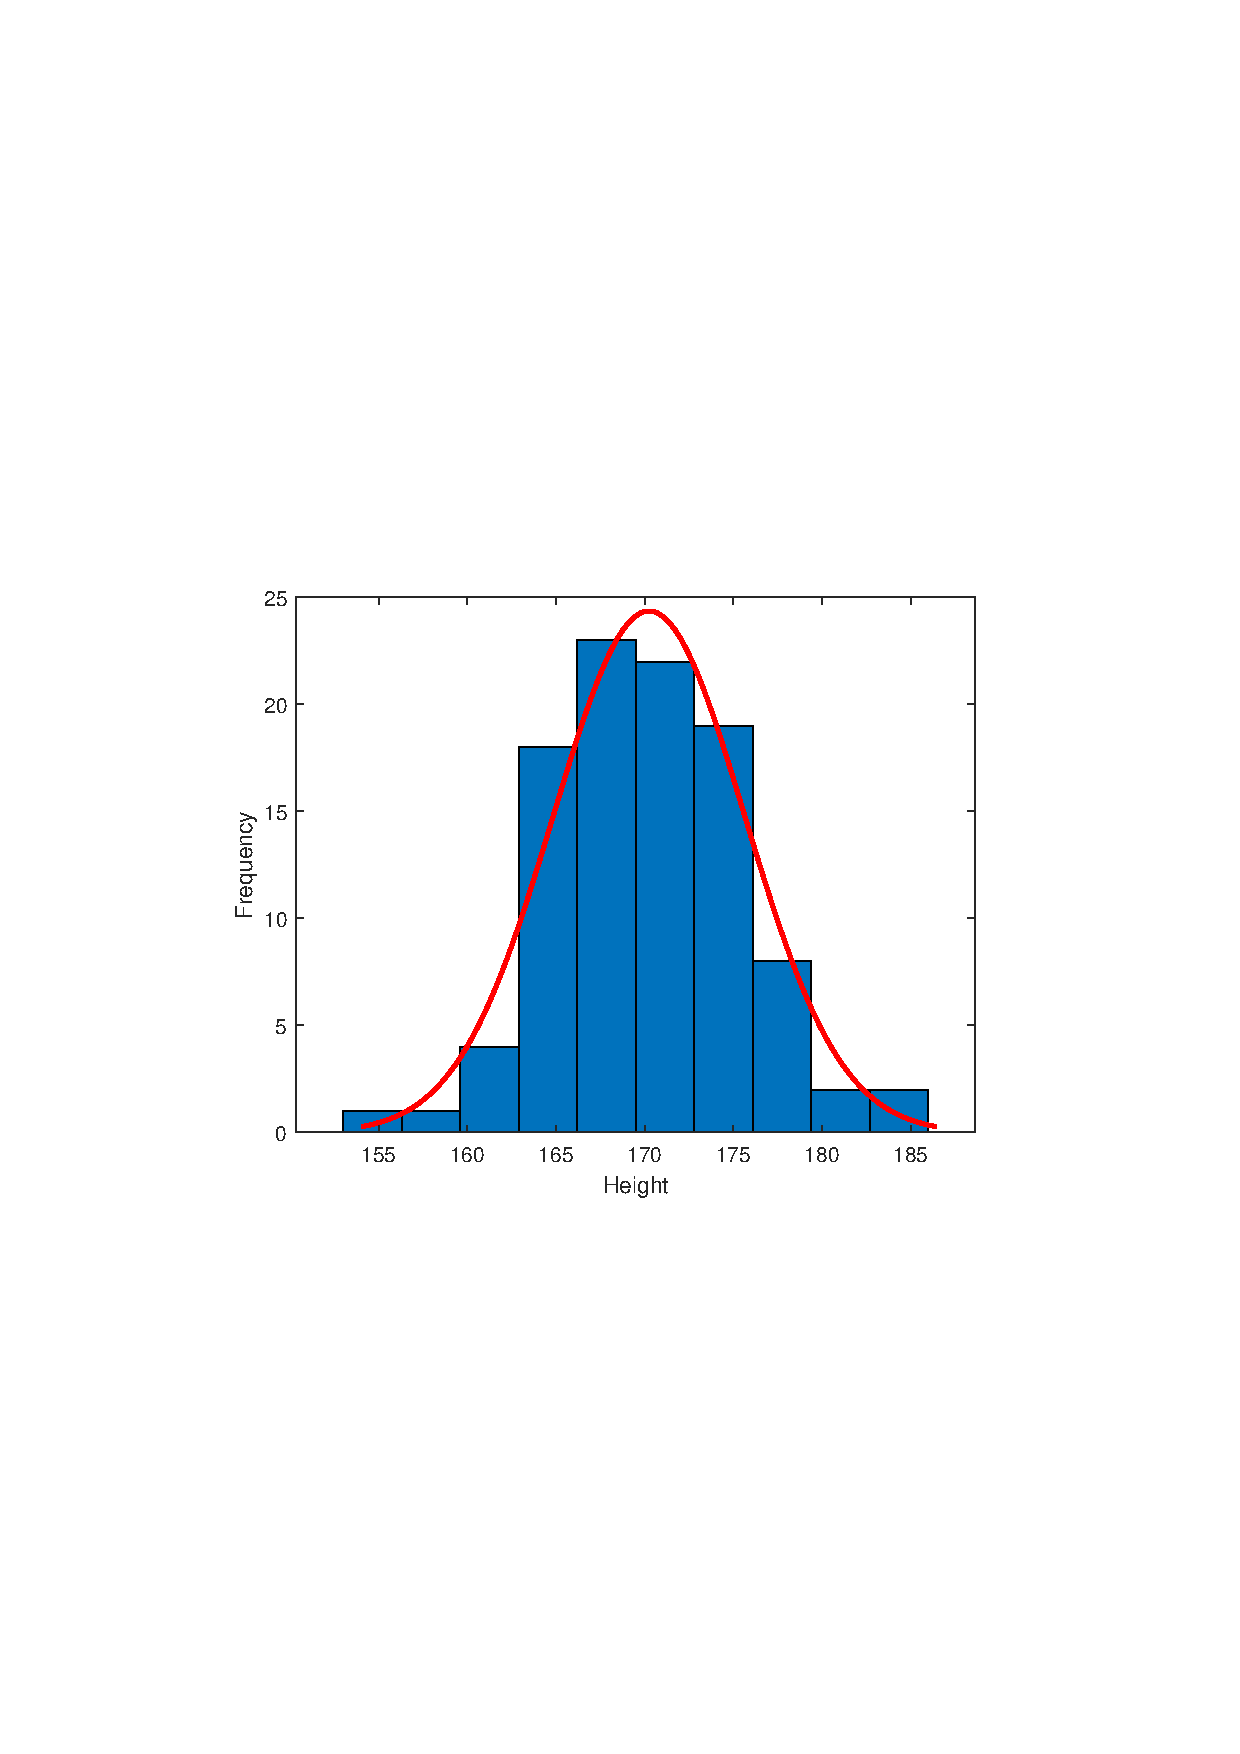
\includegraphics[width=0.47\textwidth,trim={3.09cm 9.295cm 3.09cm 9.295cm},clip]{fig/ex6_height_histfit.pdf}
    }
    \subfigure[体重分布]{
        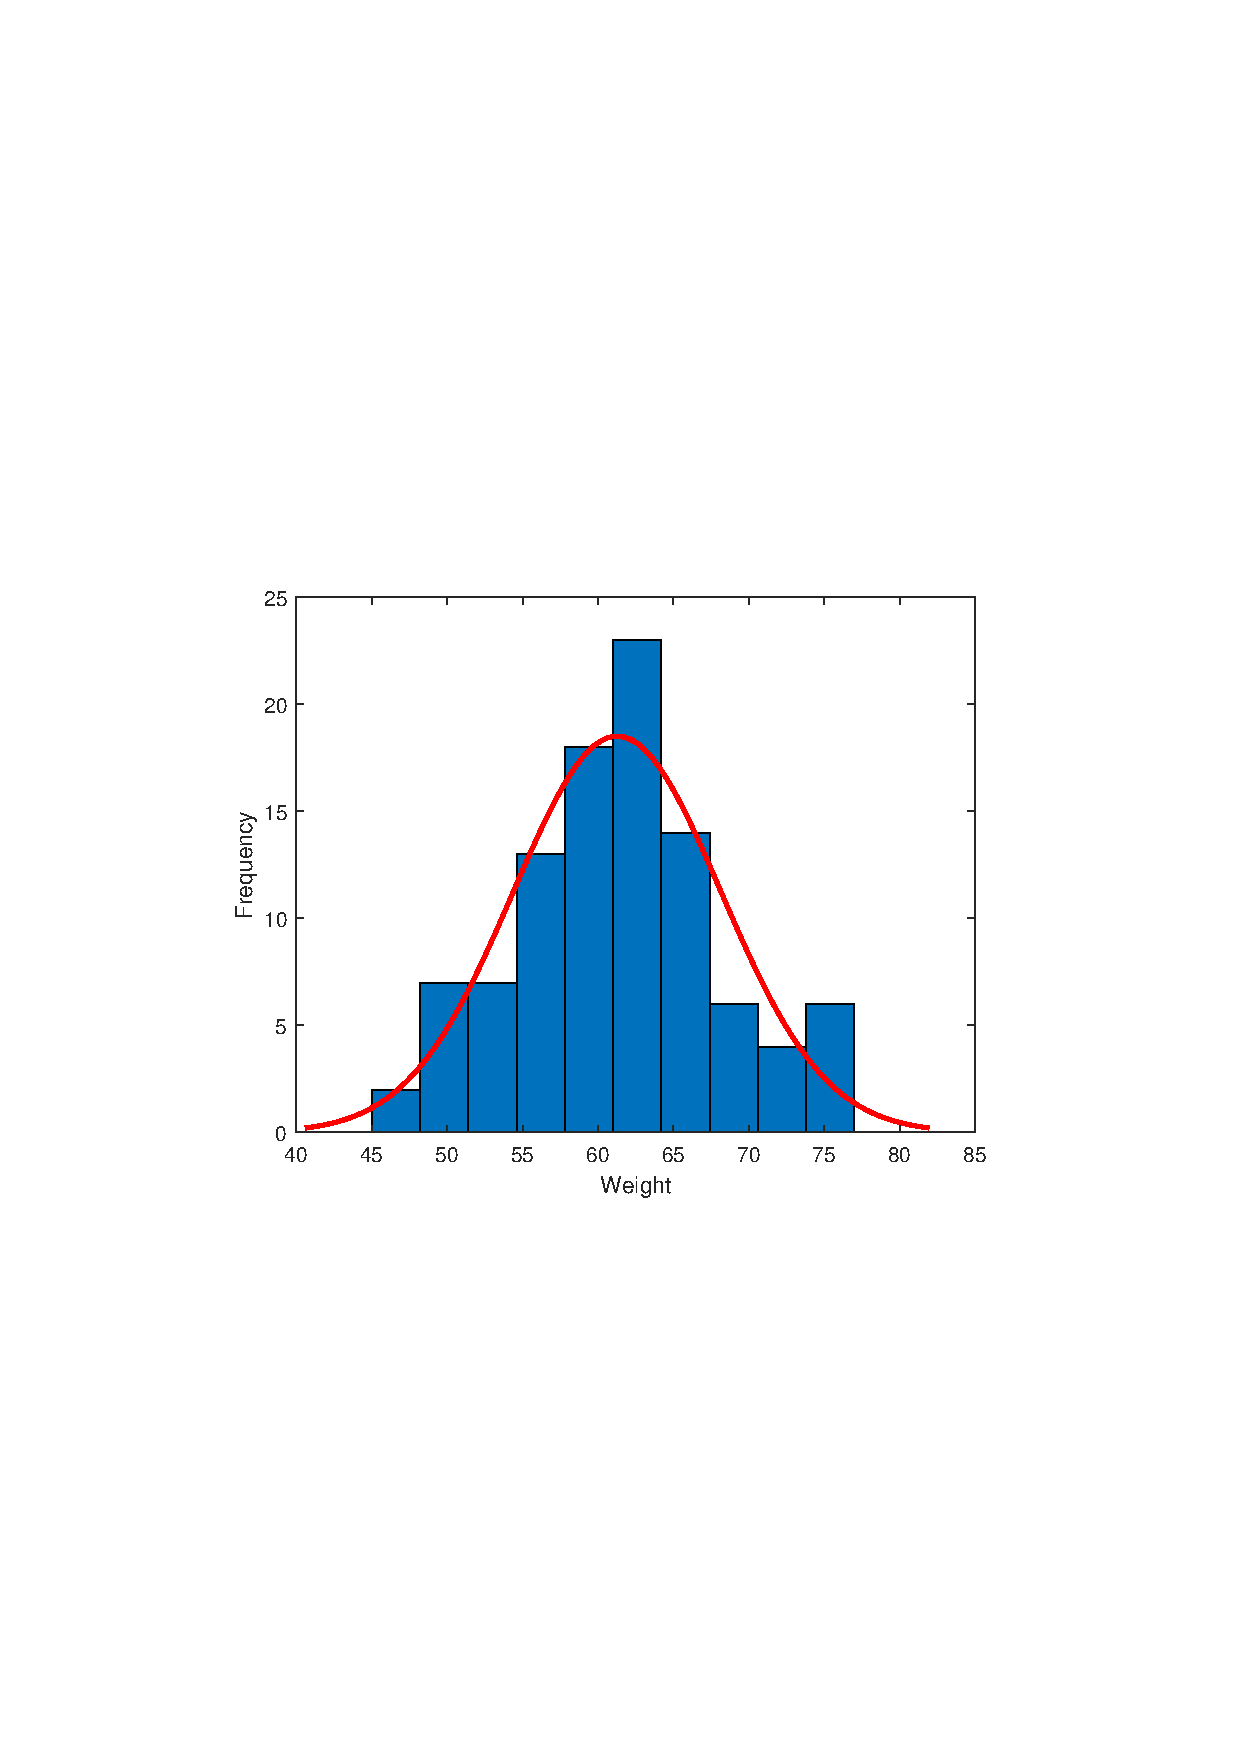
\includegraphics[width=0.47\textwidth,trim={3.09cm 9.295cm 3.09cm 9.295cm},clip]{fig/ex6_weight_histfit.pdf}
    }
    \caption{学生身高和体重的频率分布直方图及拟合的正态曲线}
    \label{fig:ex6_histfit}
\end{figure}

\paragraph{第(2)问} 在默认的显著性水平(0.05)下,身高和体重两个总体的参数估计如\Cref{tab:ex6_normfit},其中包括均值和方差的点估计和区间估计。在不同的显著性水平下,身高和体重的置信区间如\Cref{fig:ex6_height_alpha}和\Cref{fig:ex6_weight_alpha}。

\begin{table}[H]
    \centering
    \caption{身高和体重分布的参数估计}
    \label{tab:ex6_normfit}
    \begin{tabular}{c|ccccc}
        \toprule
        指标 & 均值点估计 & 标准差点估计 & 均值区间估计 &
        标准差区间估计\tabularnewline
        \midrule
        身高 (cm) & 170.25 & 5.40 & [169.18, 171.32] & [4.74,
        6.28]\tabularnewline
        体重 (kg) & 61.27 & 6.89 & [59.90, 62.64] & [6.05,
        8.01]\tabularnewline
        \bottomrule
    \end{tabular}
\end{table}

\begin{figure}[t]
    \centering
    \subfigure[均值置信区间]{
        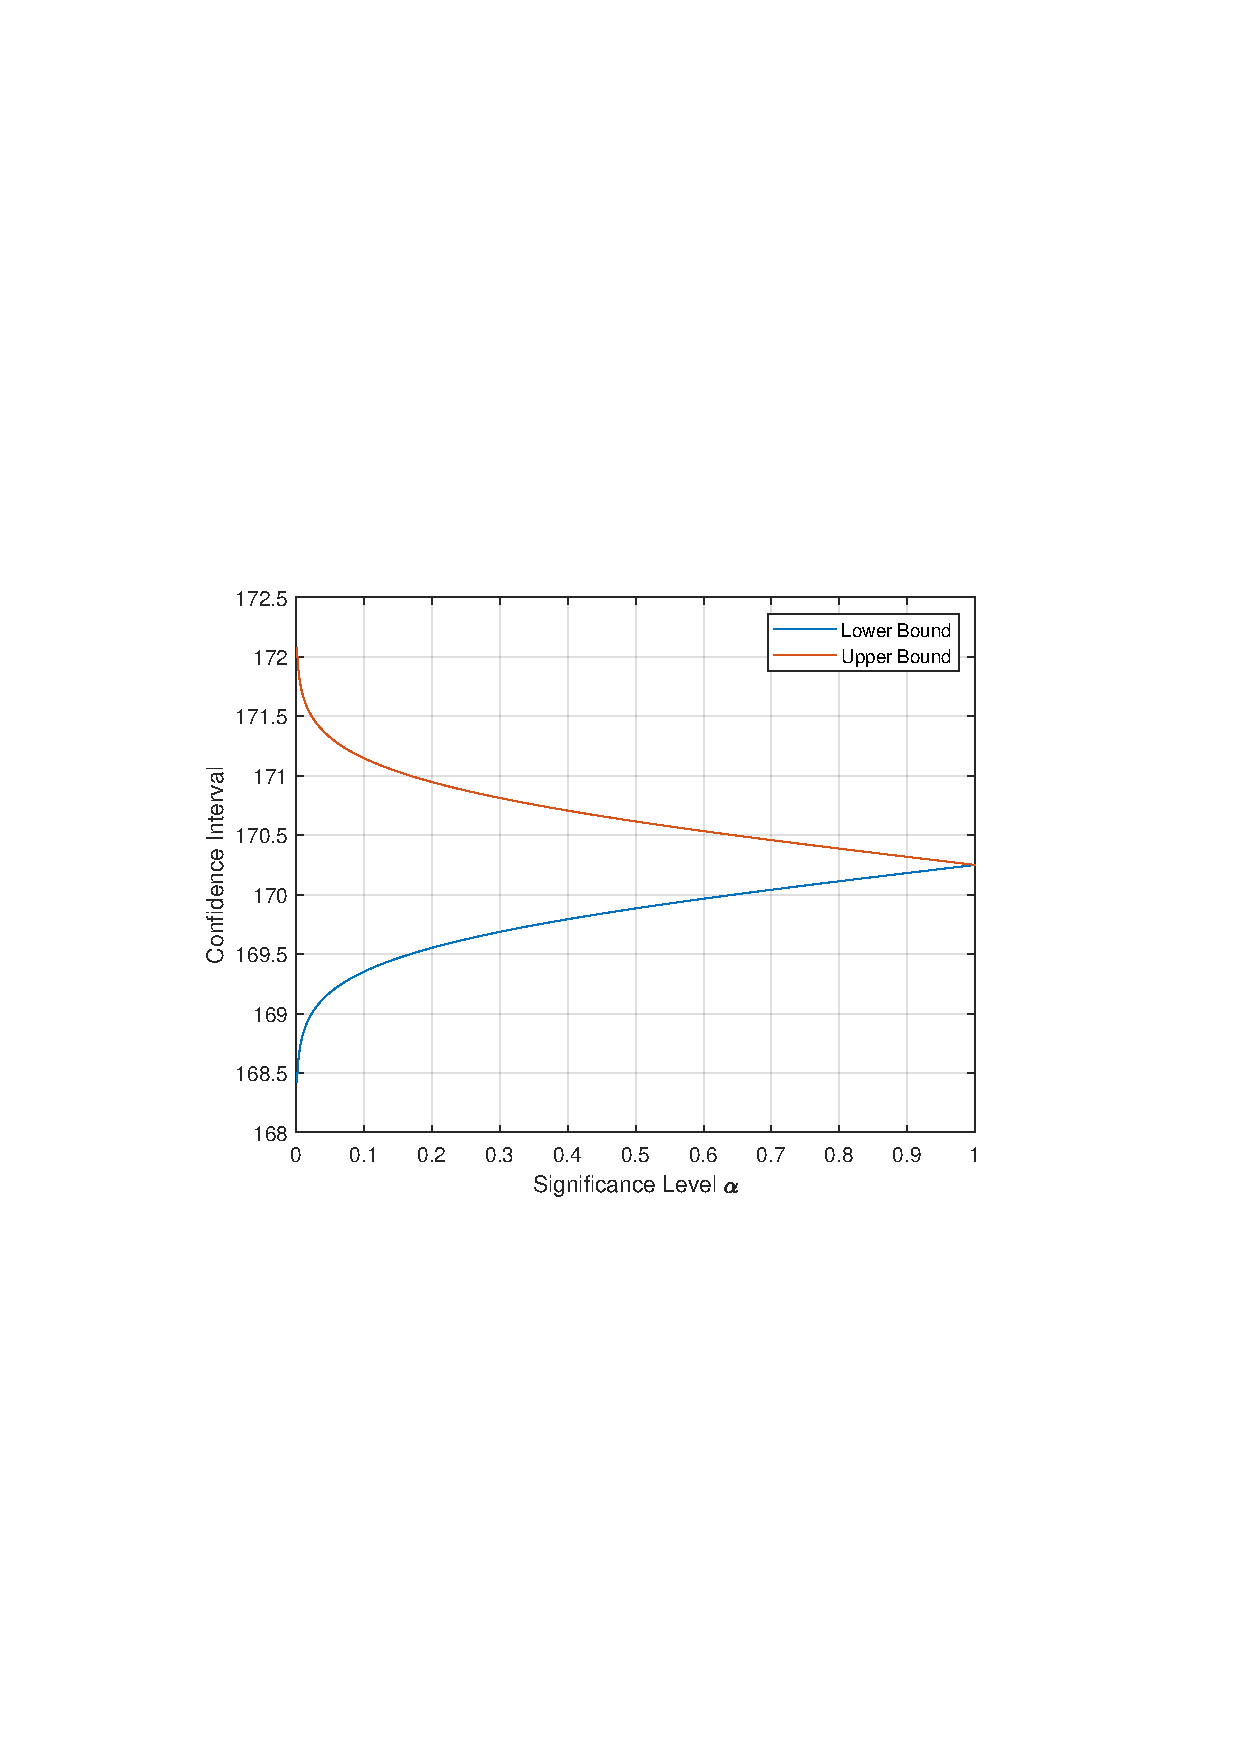
\includegraphics[width=0.47\textwidth,trim={3.09cm 9.295cm 3.09cm 9.295cm},clip]{fig/ex6_height_mu_alpha.pdf}
    }
    \subfigure[方差置信区间]{
        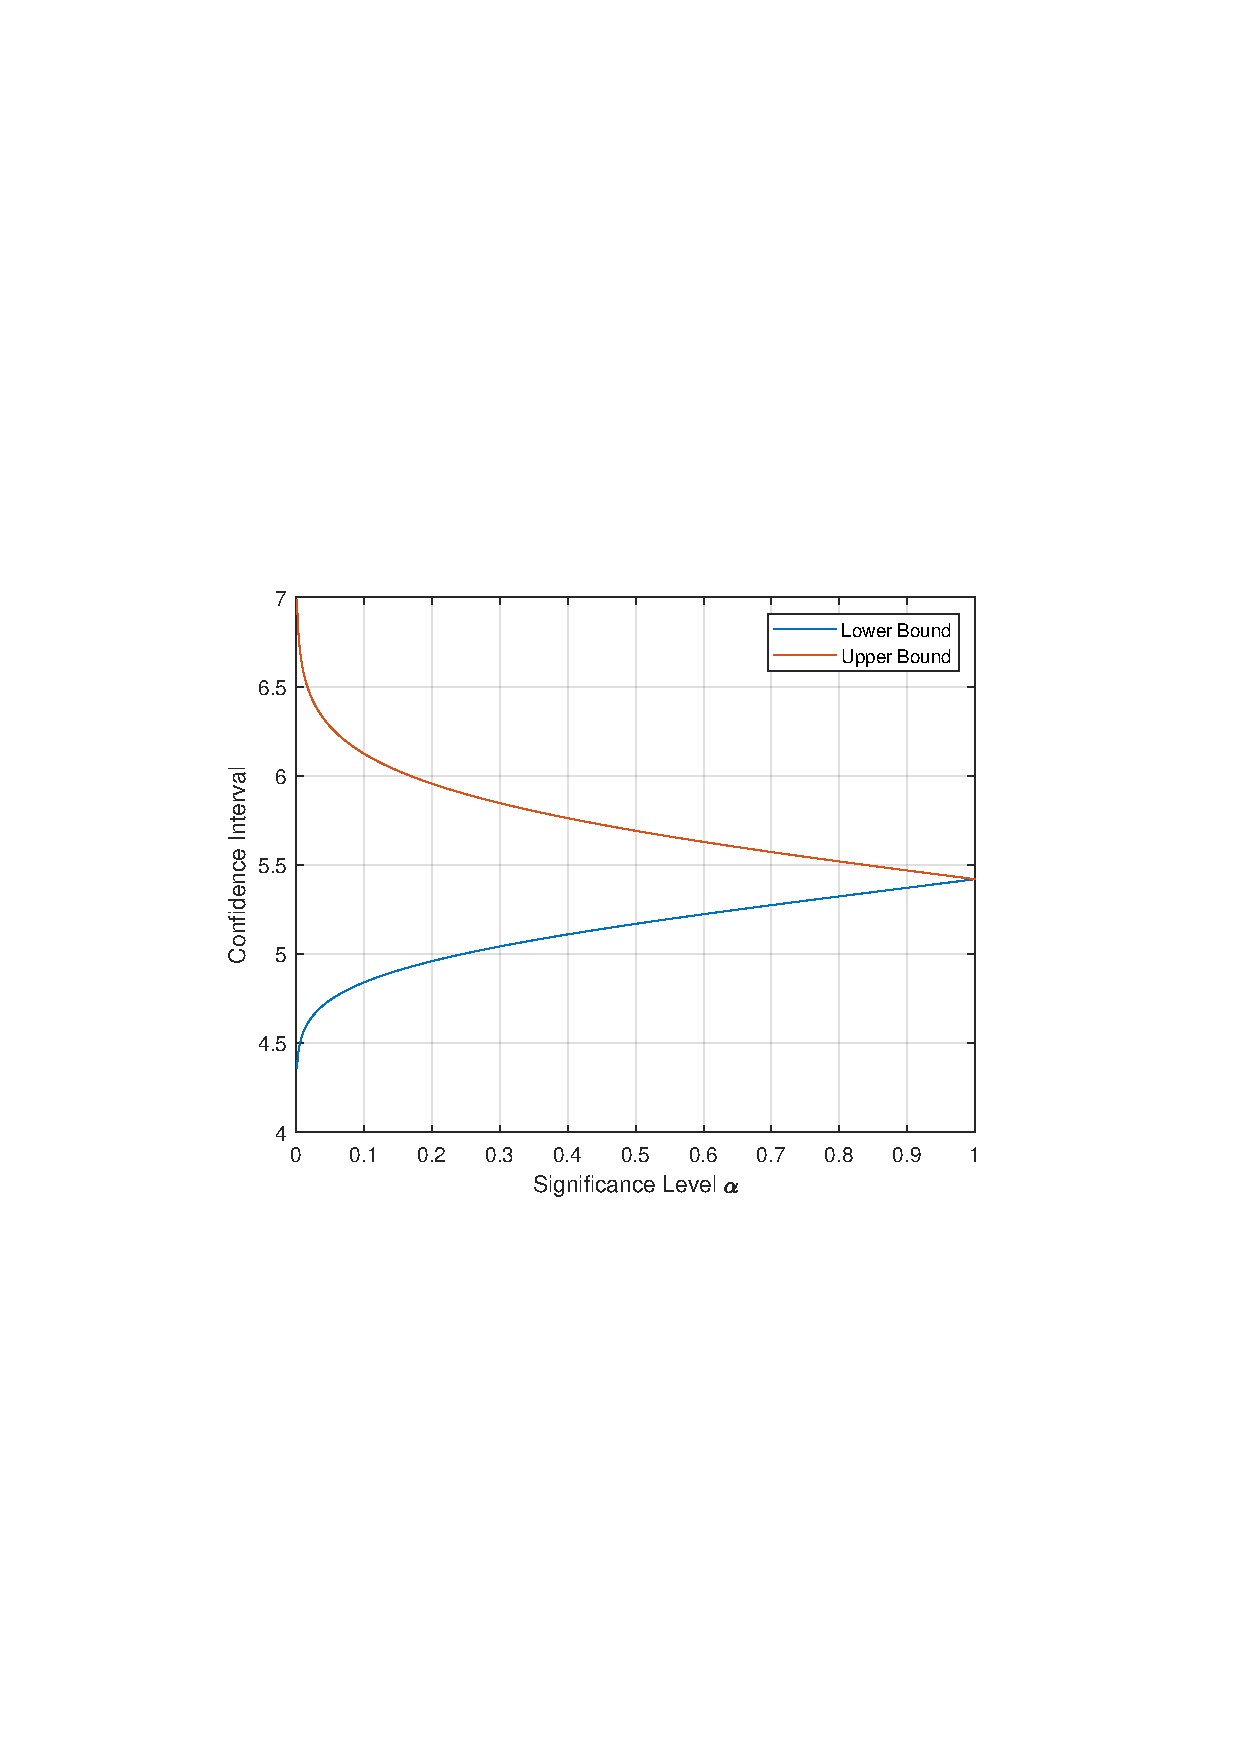
\includegraphics[width=0.47\textwidth,trim={3.09cm 9.295cm 3.09cm 9.295cm},clip]{fig/ex6_height_sigma_alpha.pdf}
    }
    \caption{不同的显著性水平下,身高的总体均值和方差的置信区间}
    \label{fig:ex6_height_alpha}
\end{figure}

\begin{figure}[t]
    \centering
    \subfigure[均值置信区间]{
        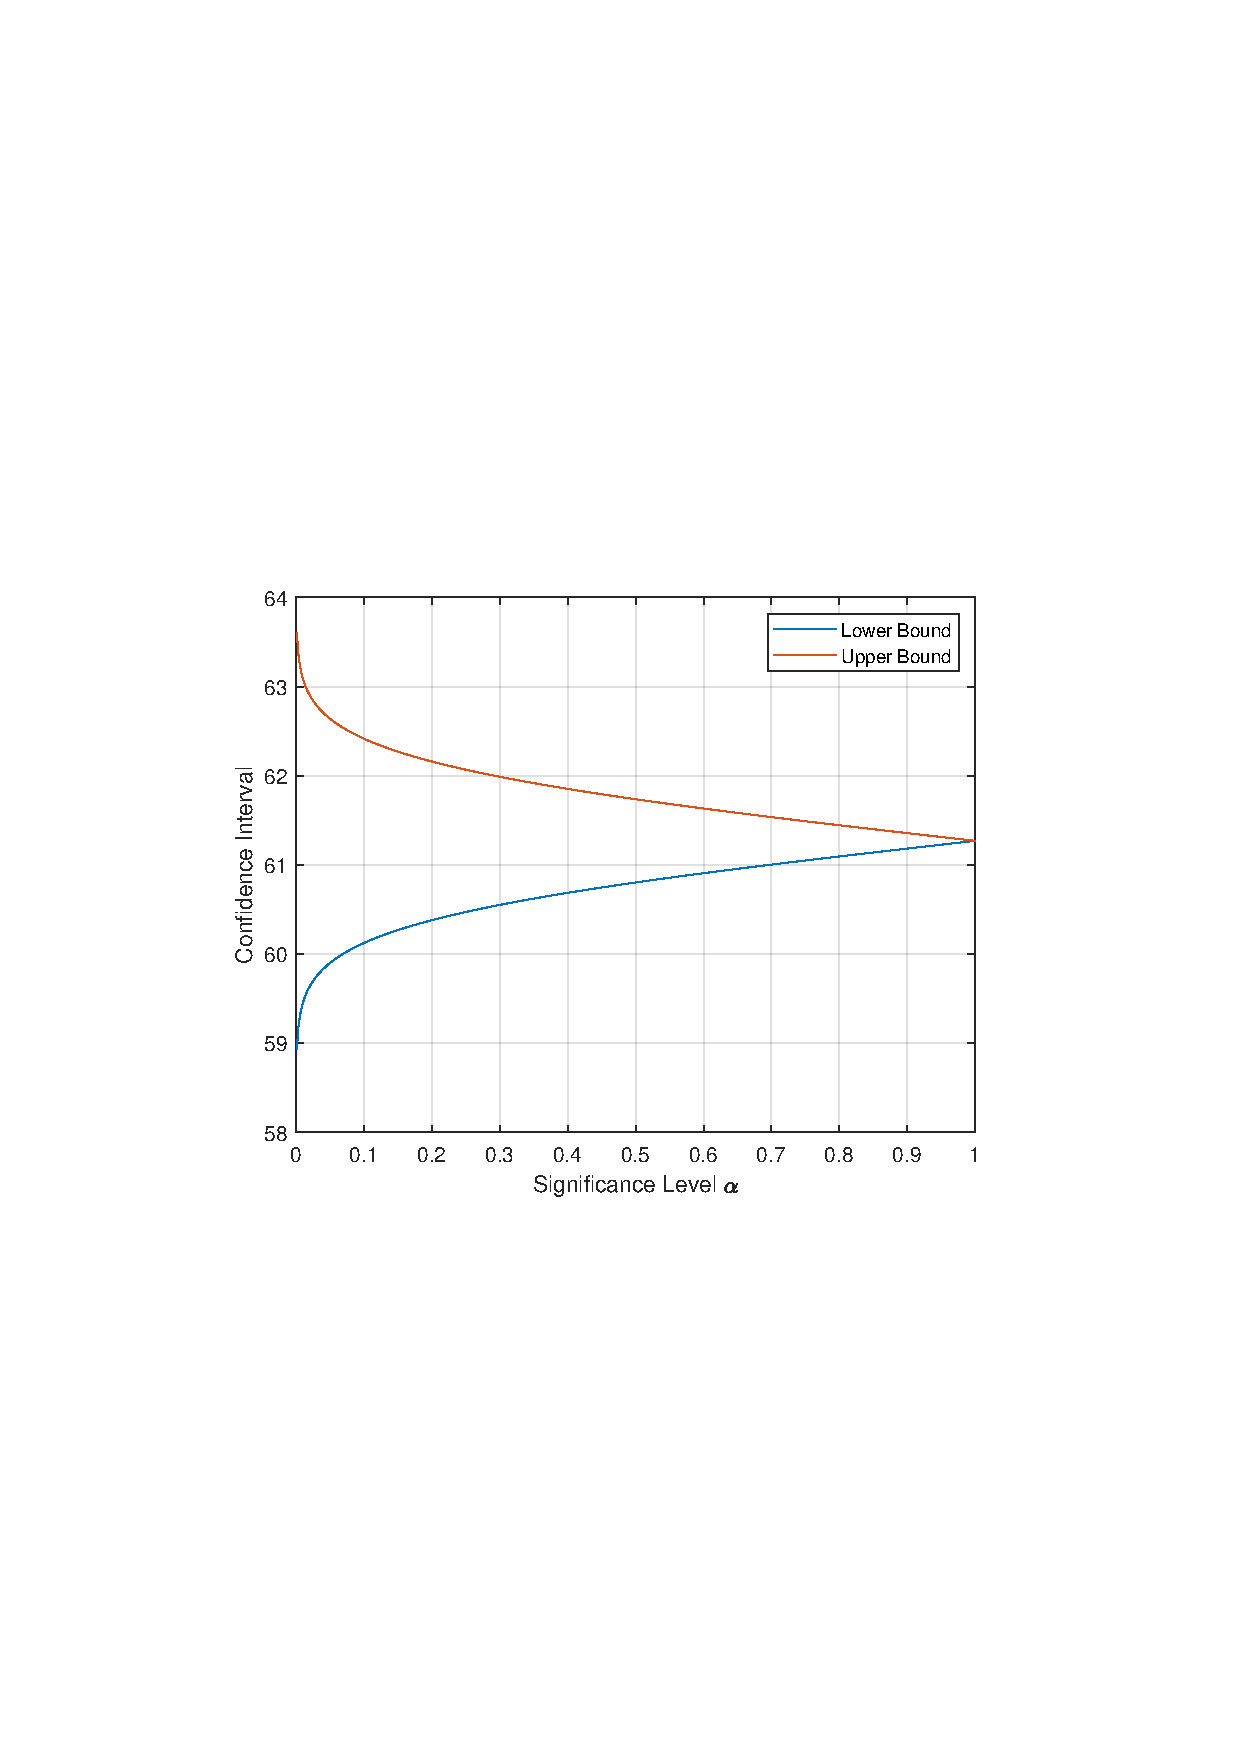
\includegraphics[width=0.47\textwidth,trim={3.09cm 9.295cm 3.09cm 9.295cm},clip]{fig/ex6_weight_mu_alpha.pdf}
    }
    \subfigure[方差置信区间]{
        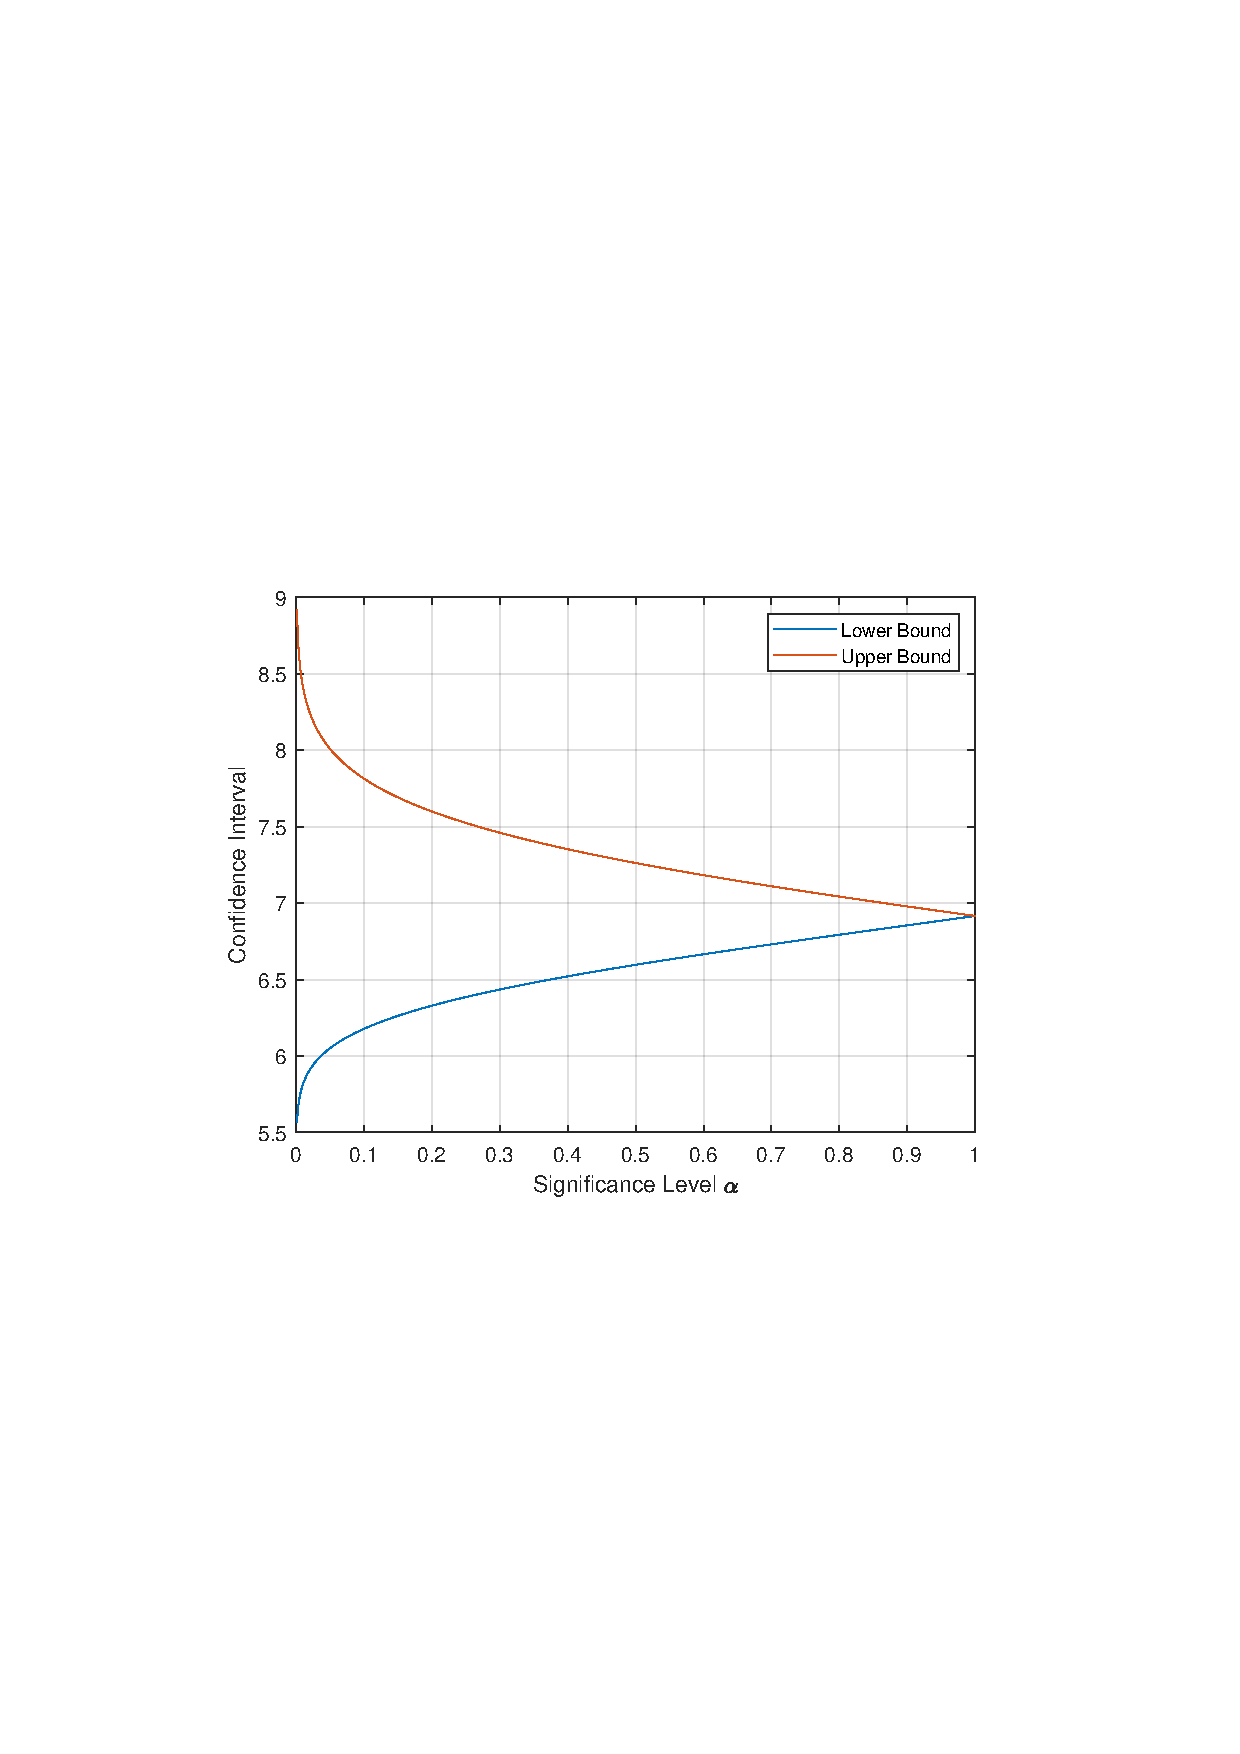
\includegraphics[width=0.47\textwidth,trim={3.09cm 9.295cm 3.09cm 9.295cm},clip]{fig/ex6_weight_sigma_alpha.pdf}
    }
    \caption{不同的显著性水平下,体重的总体均值和方差的置信区间}
    \label{fig:ex6_weight_alpha}
\end{figure}

\paragraph{第(3)问} 在默认的显著性水平(0.05)下,经过$t$检验,身高总体的原假设不成立,体重总体的原假设成立,由此可以断定,近10年来,学生的平均身高发生了明显变化,而平均体重无明显变化。

\subsubsection{结果分析}

从\Cref{fig:ex6_histfit}可以看出,在较大的样本量下,学生的身高和体重近似服从正态分布,这与概率论的中心极限定理相吻合。

从\Cref{fig:ex6_height_alpha}和\Cref{fig:ex6_weight_alpha}可以看出,当显著性水平趋于0时,置信区间长度趋于无穷;当显著性水平趋于1时,置信区间长度趋于0,收敛到点估计值;随着显著性水平的增加,即置信概率的降低,参数的置信区间随之缩小。计算结果与理论分析相符。

\subsubsection{结论}

在95\%的置信概率下,全校学生的身高和体重均服从正态分布,如\Cref{fig:ex6_histfit}。

全校学生的平均身高为170.25厘米,平均体重为61.27千克,在95\%的置信概率下,平均身高处于置信区间[169.18, 171.32]内,平均体重处于置信区间[59.90, 62.64]内。

在95\%的置信概率下,近10年来,学生的平均身高发生了明显变化,而平均体重无明显变化。
